\documentclass[12pt]{exam}
\usepackage{amsmath}
\usepackage{amssymb}
\usepackage{graphicx}
\usepackage{enumitem}
\usepackage{amsfonts}
\usepackage{amssymb}
\usepackage{ifthen}
\usepackage{geometry}
\noprintanswers

\usepackage{tikz}
\usetikzlibrary{shapes,backgrounds}

\usepackage{framed}

\addtolength{\textheight}{3.5cm}
\addtolength{\topmargin}{-0.8cm}
\addtolength{\textwidth}{2.5cm}
\addtolength{\oddsidemargin}{-1.5cm}
\addtolength{\evensidemargin}{-1.5cm}
\setlength\parindent{0pt}
\setlength{\parskip}{1em}

\newcommand {\DS} [1] {${\displaystyle #1}$}
\newcommand{\vv}{\vspace{.2cm}}

\newcommand{\R}{\mathbb{R}}
\newcommand{\Q}{\mathbb{Q}}
\newcommand{\Z}{\mathbb{Z}}
\newcommand{\N}{\mathbb{N}}

\pagestyle{empty}


%============================================
%137 COLOUR PALETTE
%============================================

\definecolor{137cp1}{RGB}{13, 33, 161}
\definecolor{137cp2}{RGB}{51, 161, 253}
\definecolor{137cp3}{RGB}{255, 67, 101}
\definecolor{137cp4}{RGB}{232, 144, 5}

% to use colours easily
\newcommand{\azul}[1]{{\color{blue} #1}}
\newcommand{\rojo}[1]{{\color{red} #1}}
 
% box in red and blue in math and outside of math
\newcommand{\cajar}[1]{\boxed{\mbox{\rojo{ #1}}}}
\newcommand{\majar}[1]{\boxed{\rojo{ #1}}}
\newcommand{\cajab}[1]{\boxed{\mbox{\azul{ #1}}}}
\newcommand{\majab}[1]{\boxed{\azul{ #1}}}

%============================================
%HYPERLINKS
%============================================

\usepackage{hyperref}
\hypersetup{colorlinks}
\hypersetup{urlcolor=137cp3, linkcolor=137cp1}

%============================================
%Commands used only for this file
%============================================


\newcommand*\circled[1]{\tikz[baseline=(char.base)]{
            \node[shape=circle,draw,inner sep=2pt] (char) {#1};}}

%%%%%%%%%%%%%%%%%%%%%%%%%%%%%%%%%%%%%%%%%


\begin{document}

{\large
	\begin{center}
		{\bf MAT 137Y: Calculus with proofs}\\
		{\bf Assignment 10} \\
		{\bf Due on Thursday, April 8 by 11:59pm via Crowdmark}
	\end{center}
}

\begin{quotation}
{\bf Instructions:}
	\begin{itemize}
		\item	 You will need to submit your solutions electronically via Crowdmark.   \href{https://www.math.toronto.edu/~alfonso/137/PS/137_CM.html}{See MAT137 Crowdmark help page for instructions}.  Make sure you understand how to submit and that you try the system ahead of time.  If you leave it for the last minute and you run into technical problems, you will be late.  There are no extensions for any reason.
		\item You may submit individually or as a team of two students.  See the link above for more details.
		\item  You will need to submit your answer to each question separately.
		\item  This problem set is based on roughly the first half of Unit 14.
	\end{itemize}
\end{quotation}

\begin{enumerate}

\item Construct a power series whose interval of convergence is exactly \DS{[0,3]}. 

\emph{Note:}  This should go without saying, but it is not enough to write down the power series: you also need to \emph{prove} that its interval of convergence \emph{is} \DS{[0,3].}

\emph{Solution:}

Let's take power series $$f(x) = \sum_{n = 1}^{\infty} \frac{(2x-3)^n}{n^2 3^n}$$

I will now proof that the interval of convergence of this power series is [0, 3]

\emph{Proof:}

Assume $t = 2x - 3$. Then the power series could be rewritten as:

$$f(t) = \sum_{n = 1}^{\infty} \frac{t^n}{n^2 3^n}$$

In order to use ratio test, let's call $a_n =  \frac{t^n}{n^2 3^n}$

\begin{align*}
	L &= \lim_{n \to \infty} \frac{|a_{n + 1}|}{|a_n|} \qquad\mbox{ (Ratio Test) } \\
	&= \lim_{n \to \infty} \frac{|\frac{t^{n + 1}}{(n + 1)^2 3^{n + 1}}|}{|\frac{t^n}{n^2 3^n}|} \qquad\mbox{ (Definition of } a_n ) \\
	&= \lim_{n \to \infty} \frac{|t^{n + 1}| n^2 3^n}{ t^n(n + 1)^2 3^{n + 1}} \qquad\mbox{(Arithmetic Operation)} \\
	&= \frac{|t|}{3} \qquad( \mbox{Since } n \to \infty \mbox{ and by definition of limit})
\end{align*}

\begin{itemize}
	\item If $|t| < 3$, then $L = \frac{|t|}{3} < 1$.

	By Ratio Test, $f(t)$ is convergent.

	\item If $|t| > 3$, then $L = \frac{|t|}{3} > 1$.

	By Ratio Test, $f(t)$ is divergent.

	\item If $|t| = 3$:

	\begin{itemize}
		\item when t = 3:

		\begin{align*}
			f(3) 
			=& \sum_{n = 1}^{\infty} \frac{3^n}{n^2 3^n} \\
			=& \sum_{n = 1}^{\infty} \frac{1}{n^2}
		\end{align*}
		By P-series test, since $p=2 > 1$, this is convergent.
		
		\item when t = -3:

		\begin{align*}
			f(-3) 
			=& \sum_{n = 1}^{\infty} \frac{(-3)^n}{n^2 3^n} \\
			=& \sum_{n = 1}^{\infty} \frac{(-1)^n\cdot3^n}{n^2 3^n} \\
			=& \sum_{n = 1}^{\infty} \frac{(-1)^n}{n^2} \\
			=& \sum_{n = 1}^{\infty} (-1)^n \frac{1}{n^2}
		\end{align*}

		In order to use Alternating Series Test, we denote $b_n = \frac{1}{n^2}$. It is known that:
		\begin{itemize}
			\item $b_n > 0, \forall n$.
			\item $\{b_n\}$ is decreasing.
			\item $\lim_{n \to \infty} b_n = 0$.
		\end{itemize}

		Therefore, $\sum_{n = 1}^{\infty} (-1)^n \frac{1}{n^2}$ is convergent.
	\end{itemize}
\end{itemize}

Therefore, $f(t)$ is convergent when $|t| \leq 3$.

Let's take back x. Then, $f(x)$ is convergent when $|2x - 3| \leq 3$. Solve it, we can get $x \in [0, 3] \blacksquare$

\newpage

\item Is it possible for a power series to be conditionally convergent at two different points?  Prove it.

\emph{Solution:}

WTS: There exists a power series to be conditionally convergent at two different points.

Let's take power series $$h(x) = \sum_{n = 1}^{\infty} \frac{(-1)^n\cdot x^{2n}}{3^{2n}\cdot n}= \sum_{n = 1}^{\infty} \frac{(-1)^n}{n}(\frac{x}{3})^{2n}$$

I will now proof that this power series to be conditionally convergent at $x=3$ and $x=-3$.

\emph{Proof:}

In order to use ratio test, let's call $a_n =  \frac{(-1)^n}{n}(\frac{x}{3})^{2n}$

\begin{align*}
	L &= \lim_{n \to \infty} \frac{|a_{n + 1}|}{|a_n|} \qquad\mbox{ (Ratio Test) } \\
	&= \lim_{n \to \infty} \frac{|\frac{(-1)^{n+1}}{(n+1)}(\frac{x}{3})^{2(n+1)}|}{|\frac{(-1)^n}{n}(\frac{x}{3})^{2n}|} \qquad\mbox{ (Definition of } a_n ) \\
	&= \lim_{n \to \infty} \frac{|(-1)^{n+1}n|(\frac{x}{3})^{2n+2}}{|(-1)^n(n+1)|(\frac{x}{3})^{2n}} \qquad\mbox{(Arithmetic Operation)} \\
	&= \lim_{n \to \infty} \frac{n}{n+1}\cdot (\frac{x}{3})^2 \qquad\mbox{(Arithmetic Operation)} \\
	&= \frac{x^2}{9} \qquad( \mbox{Since } n \to \infty \mbox{ and by definition of limit})
\end{align*}

\begin{itemize}
	\item If $|x| < 3$, then $L = \frac{x^2}{9} < 1$.

	By Ratio Test, $h(x)$ is convergent.

	\item If $|x| > 3$, then $L = \frac{x^2}{9} > 1$.

	By Ratio Test, $h(x)$ is divergent.

	\item If $|x| = 3$:

	\begin{itemize}
		\item When $x = 3$:

		\begin{align*}
			h(3)
			=& \sum_{n = 1}^{\infty} \frac{(-1)^n}{n}({\frac{3}{3}})^{2n}\\
			=& \sum_{n = 1}^{\infty} \frac{(-1)^n}{n}1^{2n} \\
			=& \sum_{n = 1}^{\infty} \frac{(-1)^n}{n} \\
			=& \sum_{n = 1}^{\infty} (-1)^n\frac{1}{n}
		\end{align*}
		In order to use Alternating Series Test, we denote $b_n = \frac{1}{n}$. It is known that:
		\begin{itemize}
			\item $b_n > 0, \forall n\in[1, \infty)$.
			\item $\{b_n\}$ is decreasing.
			\item $\lim_{n \to \infty} b_n = 0$.
		\end{itemize}
		
		Therefore, $\sum_{n = 1}^{\infty} (-1)^n \frac{1}{n}$ is convergent.
		
		\item When $x = -3$:

		\begin{align*}
			h(-3)
			=& \sum_{n = 1}^{\infty} \frac{(-1)^n}{n}({\frac{-3}{3}})^{2n}\\
			=& \sum_{n = 1}^{\infty} \frac{(-1)^n}{n}(-1)^{2n} \\
			=& \sum_{n = 1}^{\infty} \frac{(-1)^n}{n}\cdot1^n \\
			=& \sum_{n = 1}^{\infty} (-1)^n\frac{1}{n}
		\end{align*}

		In order to use Alternating Series Test, we denote $b_n = \frac{1}{n}$. It is known that:
		\begin{itemize}
			\item $b_n > 0, \forall n\in[1, \infty)$.
			\item $\{b_n\}$ is decreasing.
			\item $\lim_{n \to \infty} b_n = 0$.
		\end{itemize}
		

		Therefore, $\sum_{n = 1}^{\infty} (-1)^n \frac{1}{n}$ is convergent.
	\end{itemize}
	\item Since when $x = 3$ and $x=-3$, $h(3)=h(-3)=\sum_{n = 1}^{\infty} (-1)^n\frac{1}{n}$ and it is convergent.
	\begin{itemize}
	    \item We want to use definition of conditional convergent, it is known that:
	    
	        ``A convergent series $\sum_{n}^\infty a_n$ is conditionally convergent when $\sum_{n}^\infty |a_n|=\infty$".
	    
	    \item When we denote $a_n=(-1)^n\frac{1}{n}$:
	    
            We have shown $a_n$ is convergent when $x=3$ and $x=-3$.
        
        \item When add absolute value to $a_n$ as $\sum_{n=1}^\infty |a_n|$:
        \begin{align*}
            \sum_{n=1}^\infty |a_n|
            &=\sum_{n=1}^\infty |(-1)^n\frac{1}{n}| \qquad(\mbox{Definition of } a_n)\\
            &=\sum_{n=1}^\infty \frac{1}{n} \qquad\mbox{(Arithmetic Operation)}
        \end{align*}
        By P-series test, since $p=1 \leq 1$, this is divergent. By definition of divergent, we have $\sum_{n=1}^\infty |a_n|=\infty$.
	\end{itemize}
	Therefore, we have shown $\sum_{n = 1}^{\infty} (-1)^n\frac{1}{n}$ is conditionally convergent.
\end{itemize}

Therefore, $h(x)$ is convergent when $|x| \leq 3$ as $x\in[-3,3]$ and conditionally convergent for $x=3$ and $x=-3$ (two different points). $\blacksquare$

\newpage

\item Let \DS{f(x) = x^{100} e^{2x^5} \cos ( x^2) }.  Calculate \DS{f^{(137)}(0)}.   

You may leave your answer indicated in terms of sums, products, and quotients of rational numbers and factorials, but not in terms of sigma notation.  For example, it is okay to leave your answer as
	$$
		 15 + \frac{4!}{10} - \frac{2 \cdot 7!}{13 \cdot 13!}
	$$ 
Notice that this is just an example, not the actual answer.	

\emph{Hint:}  Use Taylor series.  

\emph{Proof:}

Since we want to find $f^{(137)}(0)$, we let $a=0\in\R$.

Let $f(x) = x^{100} e^{2x^5} \cos ( x^2)$.

We know $f$ is analytic, since $f$ is the product of a polynomial, a composition of $e$ and a polynomial, and a composition of $\cos$ and a polynomial. Using definition of Maclaurin series as ``Taylor series at $0$":
$$
    f(x)=\sum_{n=0}^\infty \frac{f^{(n)}(0)}{n!}x^n \qquad\circled{1}
$$

We know from four main Maclaurin series that:
\begin{align*}
    e^x &= \sum_{n=0}^\infty \frac{x^n}{n!}\quad\mbox{for all }x\\
    \cos x &= \sum_{n=0}^\infty  (-1)^n\frac{x^{2n}}{(2n)!}\quad\mbox{for all }x
\end{align*}
Then we express $f(x)$ as new form:
\begin{align*}
    f(x) &= x^{100}\sum_{n=0}^\infty \frac{(2x^5)^n}{n!}\sum_{n=0}^\infty  (-1)^n\frac{(x^2)^{2n}}{(2n)!} \\
    &= x^{100}\sum_{n=0}^\infty \frac{2^n\cdot x^{5n}}{n!}\sum_{n=0}^\infty  (-1)^n\frac{x^{4n}}{(2n)!} \qquad\circled{2}
\end{align*}
Since the Maclaurin series of $f$ is unique, so two equation \circled{1} and \circled{2} must be the same. Then we will have the same coefficient of $x^{137}$ in both \circled{1} and \circled{2} and we use $n_1$ to replace $n$ in $\sum_{n=0}^\infty \frac{2^n\cdot x^{5n}}{n!}$ and we use $n_2$ to replace $n$ in $\sum_{n=0}^\infty  (-1)^n\frac{x^{4n}}{(2n)!}$ then we can get one new equation:
\begin{align*}
    5n_1+4n_2&=137-100
\end{align*}
The only natural number solution to $5n_1+4n_2=137-100=37$ are $n_1=1,n_2=8$ and $n_1=5,n_2=3$
\begin{itemize}
    \item When $n_1=1,n_2=8$:
    
    We solve coefficient for $x^{137}$ in \circled{2}:
    $$
        x^{100}\cdot\frac{2^1}{1!}x^{5}\cdot\frac{(-1)^8}{(2\cdot8)!}x^{32}=2\cdot\frac{1}{16!}x^{(100+5+32)}=\frac{2}{16!}x^{137}
    $$
    \item When $n_1=5,n_2=3$:
    
    We solve coefficient for $x^{137}$ in \circled{2}:
    $$
        x^{100}\cdot\frac{2^5}{5!}x^{25}\cdot\frac{(-1)^3}{(2\cdot3)!}x^{12}=\frac{2^5}{5!}\cdot\frac{-1}{6!}x^{(100+25+12)}=\frac{-2^5}{5!\cdot6!}x^{137}
    $$
\end{itemize}
The coefficient of $x^{137}$ are sum of different combinations as:
\begin{align*}
    \frac{f^{(137)}(0)}{137!}&=\frac{2}{16!}+\frac{-2^5}{5!\cdot6!}\\
    f^{(137)}(0)&=137![\frac{2}{16!}+\frac{-2^5}{5!\cdot6!}]\\
    f^{(137)}(0)&=\frac{2\cdot137!}{16!}-\frac{2^5\cdot137!}{5!\cdot6!}\qquad\blacksquare
\end{align*}

\newpage

\item  Let $I$ be an open interval.    Let $f$ be a function defined on $I$.  Let $a \in I$.  Assume $f$ is $C^2$ on $I$.   Assume $f'(a) = 0$.   As you know, $a$ is a candidate for a local extremum for $f$.  The ``2nd Derivative Test" says that, under these circumstances:
	\begin{itemize}
		\item  IF $f''(a)>0$, THEN $f$ has a local minimum at $a$.
		\item  IF $f''(a)<0$, THEN $f$ has a local maximum at $a$.
	\end{itemize}
	 This theorem is easier to justify, and to generalize, using Taylor polynomials.
	\begin{enumerate}
		\item  \label{qu:int} Let $P_2$ be the 2nd Taylor polynomial for $f$ at $a$.  Write an explicit formula for $P_2$.
		
			Using the idea that $f(x) \approx P_2(x)$ when $x$ is close to $a$, write an intuitive explanation for the 2nd Derivative Test.  
			
			\emph{Note:}  We are not asking for a proof yet.  Rather, we are asking for a short, simple, handwavy argument that would convince an average student that this result ``makes sense" and ``seems true".
			
			\emph{Solution}:
			
			Let $a \in I\subseteq\R$.
			
			Let $n=2\in\N$.
			
			Assume $f$ is $C^2$ on $I$.
			
			Then $f$ is $C^2$ at $a$.
			
			By 3-rd definition of Taylor polynomials, we have
			$$
			    P_2(x)=\sum_{k=0}^2 \frac{f^{(k)}(a)}{k!}(x-a)^k=f(a)+f'(a)(x-a)+\frac{f''(a)}{2}(x-a)^2
			$$
			Since we assume $f'(a) = 0$, we then have
			$$
			    P_2(x)=f(a)+0\cdot(x-a)+\frac{f''(a)}{2}(x-a)^2=f(a)+\frac{f''(a)}{2}(x-a)^2
			$$
			Then we can seen $f(a)$ as constant, $\frac{f''(a)}{2}$ as coefficient of $x^2$ and $P_2(x)$ is a quadratic function.
			
			When $f''(a)>0$, the quadratic function concave up as:
			\begin{center}
			    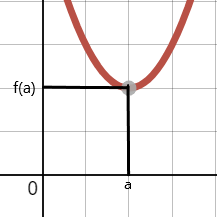
\includegraphics[scale=0.75]{Upward}
			    
			    (Red line represents $P_2(x)$)
			\end{center}
			Graphically, we have shown that $f$ has a local minimum at $a$.
			
			\newpage
			
			When $f''(a)<0$, the quadratic function concave down as:
			\begin{center}
			    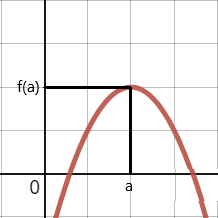
\includegraphics[scale=0.75]{Downward}
			    
			    (Red line represents $P_2(x)$)
			\end{center}
			Graphically, we have shown that $f$ has a local maximum at $a$.
			
			\newpage
			
		\item  \label{qu:pf} Now write an actual, rigorous proof for the 2nd Derivative Test.  You will need to use the first definition of Taylor polynomial (the one in terms of the limit), the definition of limit, and the definition of local extremum.
				
			\emph{Note:}  There are many other ways to prove the 2nd Derivative Test, but we want you to do it specifically this way. It will help with the next questions.
			
			\emph{Proof:}
			
			Let $a \in I\subseteq\R$.
			
			Let $n=2\in\N$.
			
		    Assume $f$ is $C^2$ on $I$.
		    
		    By definition of $C^2$, A function $f$ is called $C^2$ when $f'$ and $f''$ exist and are continuous.
			
			Then $f$ is $C^2$ at $a$ which shows $f$ is a continuous function defined at and near $a$.
			
			By 1-st definition of Taylor polynomials, we have
			$$
			    \lim_{x\to a}\frac{f(x)-P_n(x)}{(x-a)^n}=\lim_{x\to a}\frac{f(x)-P_2(x)}{(x-a)^2}=0\qquad\circled{3}
			$$
			Assume $f'(a) = 0$. From Q4a, we have shown
			$$
			    P_2(x)=f(a)+\frac{f''(a)}{2}(x-a)^2
			$$
			and use this $P_2(x)$ in $\circled{3}$, we have:
			\begin{align*}
			    \lim_{x\to a}\frac{f(x)-P_2(x)}{(x-a)^2}
			    &=\lim_{x\to a}\frac{f(x)-[f(a)+\frac{f''(a)}{2}(x-a)^2]}{(x-a)^2}\\
			    &=\lim_{x\to a}[\frac{f(x)-f(a)}{(x-a)^2}-\frac{f''(a)}{2}]\\
			    &=0
			\end{align*}
			By definition of limits, we can change
			$$
			    \lim_{x\to a}[\frac{f(x)-f(a)}{(x-a)^2}-\frac{f''(a)}{2}]=0
			$$
			into formal definition as:
			$$
			    \forall\epsilon>0, \exists\delta>0 \mbox{ s.t } 0<\vert{x-a}\vert<\delta\implies\vert{\frac{f(x)-f(a)}{(x-a)^2}-\frac{f''(a)}{2}}\vert<\epsilon
			$$
			\begin{itemize}
			    \item Case One - $f''(a)>0$:
			        
			        Take $\epsilon=\frac{f''(a)}{2}>0$.
			        
			        Then by formal definition of Taylor polynomial we will have
			        \begin{align*}
			            \exists\delta>0 \mbox{ s.t } 0<\vert{x-a}\vert<\delta&\implies\vert{\frac{f(x)-f(a)}{(x-a)^2}-\frac{f''(a)}{2}}\vert<\frac{f''(a)}{2}\\
			            &\implies\frac{-f''(a)}{2}<\frac{f(x)-f(a)}{(x-a)^2}-\frac{f''(a)}{2}<\frac{f''(a)}{2}\\
			            &\implies\frac{-f''(a)}{2}+\frac{f''(a)}{2}<\frac{f(x)-f(a)}{(x-a)^2}<\frac{f''(a)}{2}+\frac{f''(a)}{2}\\
			            &\implies0<\frac{f(x)-f(a)}{(x-a)^2}<f''(a)
			        \end{align*}
			        Since we know $(x-a)^2>0$, we will have
			        \begin{align*}
			            \exists\delta>0 \mbox{ s.t } 0<\vert{x-a}\vert<\delta
			            &\implies\frac{f(x)-f(a)}{(x-a)^2}>0\\
			            &\implies f(x)-f(a)>0\qquad((x-a)^2>0)\\
			            &\implies f(x)>f(a)\\
			            &\implies f(x)\geq f(a)
			        \end{align*}
			        Thus by definition of local minimum as
			        $$
			            \exists\delta>0 \mbox{ s.t } 0<\vert{x-a}\vert<\delta\implies f(x)\geq f(a)
			        $$
			        I've showed $f$ has a local minimum at $a$.
			    \item Case Two - $f''(a)<0$:
			    
			        Take $\epsilon=\frac{-f''(a)}{2}>0$.
			        
			        Then by formal definition of Taylor polynomial we will have
			        \begin{align*}
			            \exists\delta>0 \mbox{ s.t } 0<\vert{x-a}\vert<\delta&\implies\vert{\frac{f(x)-f(a)}{(x-a)^2}-\frac{f''(a)}{2}}\vert<\frac{-f''(a)}{2}\\
			            &\implies\frac{f''(a)}{2}<\frac{f(x)-f(a)}{(x-a)^2}-\frac{f''(a)}{2}<\frac{-f''(a)}{2}\\
			            &\implies\frac{f''(a)}{2}+\frac{f''(a)}{2}<\frac{f(x)-f(a)}{(x-a)^2}<\frac{-f''(a)}{2}+\frac{f''(a)}{2}\\
			            &\implies f''(a)<\frac{f(x)-f(a)}{(x-a)^2}<0
			        \end{align*}
			        Since $(x-a)^2>0$, we will have
			        \begin{align*}
			            \exists\delta>0 \mbox{ s.t } 0<\vert{x-a}\vert<\delta
			            &\implies\frac{f(x)-f(a)}{(x-a)^2}<0\\
			            &\implies f(x)-f(a)<0\qquad((x-a)^2>0)\\
			            &\implies f(x)<f(a)\\
			            &\implies f(x)\leq f(a)
			        \end{align*}
			        Thus by definition of local maximum as
			        $$
			            \exists\delta>0 \mbox{ s.t } 0<\vert{x-a}\vert<\delta\implies f(x)\leq f(a)
			        $$
			        I've showed $f$ has a local maximum at $a$.\qquad $\blacksquare$
			\end{itemize}
			
			\newpage
	
		\item \label{qu:conj} What happens if $f''(a)=0$?     In that case, we look at $f^{(3)}(a)$;  if it is also $0$, then we look at $f^{(4)}(a)$, and we keep looking till we find one derivative that is not $0$ at $a$.   
		
		More specifically, assume that $f$ is $C^n$ at $a$ for some natural number $n \geq 2$ and that $f^{(n)}(a)$ is the smallest derivative  that is not $0$ at $a$.   In other words, $f^{(k)}(a) =0$ for $ 1 \leq k < n$ but $f^{(n)}(a) \neq 0$.
		
		Using the same ideas as in Question \ref{qu:int}, complete the following statements, and give an intuitive explanation for them:
			\begin{itemize}
				\item  IF ..., THEN $f$ has a local minimum at $a$.
				\item  IF ..., THEN $f$ has a local maximum at $a$.
				\item  IF ..., THEN $f$ does not have a local extremum at $a$.
			\end{itemize}
		When you complete this, you will have come up with a new theorem.  Let's call it the ``Beyond-the-2nd-derivative Test".   Make sure your theorem takes care of all possible cases.  
		
		\emph{Solution:}
		    \begin{itemize}
				\item  IF $n$ is even and $f^{(n)}(a)>0$, THEN $f$ has a local minimum at $a$.
				\item  IF $n$ is even and $f^{(n)}(a)<0$, THEN $f$ has a local maximum at $a$.
				\item  IF $n$ is odd, THEN $f$ does not have a local extremum at $a$.
			\end{itemize}
		    Let $a \in I\subseteq\R$.
			
			Let $n\geq2\in\N$.
			
			Assume $f$ is $C^n$ on $I$.
			
			By 3-rd definition of Taylor polynomials, we have
			\begin{align*}
			    P_n(x)&=\sum_{k=0}^n \frac{f^{(k)}(a)}{k!}(x-a)^k\\
			    &=f(a)+f^{(1)}(a)(x-a)+\frac{f^{(2)}(a)}{2!}(x-a)^2+\cdots+\frac{f^{(n-1)}(a)}{(n-1)!}(x-a)^{n-1}+\frac{f^{(n)}(a)}{n!}(x-a)^n
			\end{align*}
			Since we assume $f^{(1)}(a)=0,f^{(2)}(a)=0,\cdots,f^{(n-1)}(a)=0$, we then have:
			$$
			    P_n(x)=f(a)+0\cdot(x-a)+\cdots+0\cdot(x-a)^{n-1}+\frac{f^{(n)}(a)}{n!}(x-a)^n=f(a)+\frac{f^{(n)}(a)}{n!}(x-a)^n
			$$
			Then we can seen $f(a)$ as constant, $\frac{f^{(n)}(a)}{n!}$ as coefficient of $x^n$ and the shape of $P_n(x)$ needed to be discussed based on $n$ is even or odd.
			\begin{itemize}
			    \item When $n$ is even and $f^{(n)}(a)>0$, the function $P_n(x)$ concave up as:
			        \begin{center}
			            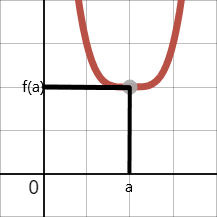
\includegraphics[scale=0.75]{Upward-n}
			    
			            (Red line represents $P_n(x)$)
			        \end{center}
			        Graphically, we have shown that $f$ has a local minimum at $a$.
			
			    \item When $n$ is even and $f^{(n)}(a)<0$, the function $P_n(x)$ concave down as:
			        \begin{center}
			            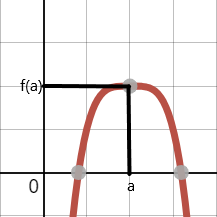
\includegraphics[scale=0.75]{Downward-n}
			    
			            (Red line represents $P_n(x)$)
			        \end{center}
			        Graphically, we have shown that $f$ has a local maximum at $a$.
			     
		        \item When $n$ is odd and $f^{(n)}(a)>0$, the function $P_n(x)$ shape will be like:
		            \begin{itemize}
		                \item When $f^{(n)}(a)>0$, the function $P_n(x)$ shape will be like:
		                    \begin{center}
			                    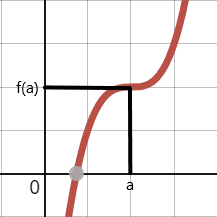
\includegraphics[scale=0.75]{Odd-Positive}
			    
			                    (Red line represents $P_n(x)$)
			                \end{center}
		                \item When $f^{(n)}(a)<0$, the function $P_n(x)$ shape will be like:
		                    \begin{center}
			                    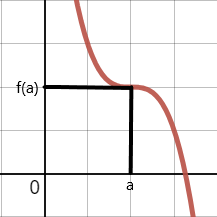
\includegraphics[scale=0.75]{Odd-Negative}
			    
			                    (Red line represents $P_n(x)$)
			                \end{center}
		            \end{itemize}
		            Graphically, we have shown that $f$ does not have a local extremum at $a$.
			\end{itemize}
		
		\newpage
		
		\item \label{qu:thm}  {\bf [Do not submit.]}  Imitate the proof in \ref{qu:pf} to prove the Beyond-the-2nd-derivative Test. 	
	\end{enumerate}

\emph{Note:}  Why did we ask you to write both a ``simple, intuitive explanation" and a ``formal proof"?  Because that is how research in mathematics often happens.  The intuitive explanation is how we come up with conjectures and discover new theorems (as in Questions \ref{qu:int} and \ref{qu:conj}).   After that, the formal proof is how we make sure the conjecture is not merely a conjecture but a true theorem (as in Questions \ref{qu:pf} and \ref{qu:thm}).   We need both.

\end{enumerate}
\end{document}
%%%%%%%%%%%%%%%%%%%%%%%%%%%%%%%%
%%%%%%%%%%%%%%%%%%%%%%%%%%%%%%%%

